\documentclass[10pt, xcolor=dvipsnames]{beamer}
%\documentclass[10pt, xcolor=dvipsnames,notes=only]{beamer}
%\mode<presentation>
%{
\usetheme{Goettingen}
%\setbeamercovered{transparent}
%} 
\usefonttheme{professionalfonts}
%\usecolortheme{beaver}

\usepackage{setspace}
\usepackage[english]{babel}
\usepackage[latin1]{inputenc}
\usepackage{times}
\usepackage[T1]{fontenc}
\usepackage{color}
\usepackage{graphicx}
\usepackage{amssymb}
\usepackage{amsthm}
\usepackage{bm}
\usepackage{rotating}
\usepackage{ccaption}
\usepackage{booktabs}
\usepackage{lscape}
\usepackage{colortbl}
\usepackage{arydshln}
\usepackage{tabularx}
\usepackage{graphics}
\usepackage{epstopdf}

\setbeamertemplate{navigation symbols}{}
\setbeamertemplate{items}[balls]

\newenvironment{changemargin}[2]{%
  \begin{list}{}{%
    \setlength{\topsep}{0pt}%
    \setlength{\leftmargin}{#1}%
    \setlength{\rightmargin}{#2}%
    \setlength{\listparindent}{\parindent}%
    \setlength{\itemindent}{\parindent}%
    \setlength{\parsep}{\parskip}%
  }%
  \item[]}{\end{list}}

\setbeamercolor{block title}{fg=white, bg=teal}
\setbeamercolor{block body}{bg=teal!25}

\author[]{Chad Jones and Dietrich Vollrath}
\institute[Intro Growth]{Introduction to Economic Growth}
\date[]{}


\title[Development]{Growth and Development}


\begin{document}
\maketitle

\section{Development accounting}
\begin{frame}{Why are some countries rich?}
What part of production - capital, productivity - is the reason some countries are rich? 
\begin{equation}
	Y_i = K_i^{\alpha} (A_i h_i L_i)^{1-\alpha}. \nonumber
\end{equation}
\begin{itemize}
	\item $K_i$ is physical capital
	\item $A_i$ is productivity
	\item $L_i$ is number of workers
	\item $h_i$ is human capital per worker...this is new but hold on
\end{itemize}
\end{frame}

\begin{frame}{GDP per capita}
Write production as
\begin{equation}
	Y_i = \left(\frac{K_i}{A_i h_i L_i} \right)^{\alpha} A_i h_i L_i, \label{EQ_Y_kahl}
\end{equation}
let 
\begin{equation}
	\frac{K_i}{Y_i} = \frac{K_i}{K_i^{\alpha} (A_i h_i L_i)^{1-\alpha}} = \left(\frac{K_i}{A_i h_i L_i} \right)^{1-\alpha}. \nonumber
\end{equation}
and divide by population ($N_i$) to get
\begin{equation}
	y_i = \left(\frac{K_i}{Y_i}\right)^{\alpha/(1-\alpha)} A_i h_i \frac{L_i}{N_i}. \label{EQ_y_i}
\end{equation}
is GDP per capita in country $i$
\end{frame}

\begin{frame}{Human capital}
Define human capital as
\begin{equation}
 	h_i = e^{\mu E_i}, \label{EQ_h_i}
\end{equation} 
\begin{itemize}
	\item $E_i$ is years of education
	\item $\mu$ is the return to each year of education (e.g. $\mu \approx 0.10$)
	\item This conforms to typical labor market studies that each year of education raises wages by about 10\%
	\item Schooling isn't the \textit{only} aspect of human capital, but we can measure it
\end{itemize}
\end{frame}

\begin{frame}{Comparing countries}
Go back and compare some country $i$ to a reference point (usually the US):
\begin{equation}
	\frac{y_i}{y_{US}} = \left[\frac{(K/Y)_i}{(K/Y)_{US}}\right]^{\alpha/(1-\alpha)} \frac{A_i}{A_{US}} \frac{h_i}{h_{US}} \frac{(L_i/N_i)}{(L_{US}/N_{US})}. \label{EQ_yi_yus}
\end{equation}
We can assess why country $i$ is richer or poorer than the US
\begin{itemize}
	\item Different capital/output ratios
	\item Different productivity levels $A_i/A_{US}$
	\item Different human capital ratios
	\item Different labor force participation
\end{itemize}
\end{frame}

\begin{frame}{Measuring productivity}
How do you measure productivity in a country?
\begin{equation}
	A_i = \frac{y_i}{\left(\frac{K_i}{Y_i}\right)^{\alpha/(1-\alpha)} h_i \frac{L_i}{N_i}}. \label{EQ_A_i}
\end{equation}
by re-arraning the equation for GDP per capita. Plug in and solve.
\end{frame}

\begin{frame}{Doing the accounting}
\begin{scriptsize}
\begin{tabular}{lccccc}
\midrule
              &                & \multicolumn{4}{c}{Components of GDP per capita:} \\ \cmidrule(lr){3-6}
              & GDP per    & Capital / & Human      & Labor force      &            \\
              & capita     & output    & capital    & partic.    & Prod.  \\
Country       & $\frac{y_i}{y_{US}}$ &  $\left[\frac{(K/Y)_i}{(K/Y)_{US}}\right]^{\frac{\alpha}{1-\alpha}}$   & $\frac{h_i}{h_{US}}$    & $\frac{(L_i/N_i)}{(L_{US}/N_{US})}$   & $\frac{A_i}{A_{US}}$\\
\midrule
%\input{tab_ch7_tab1.txt}
\csname @@input\endcsname tab_ch7_tab1.txt
\midrule
\end{tabular}
\end{scriptsize}
\end{frame}

\begin{frame}{What drives differences?}
Differences across countries in GDP per capita depend on:
\begin{itemize}
	\item Productivity - this is the main driver
	\item Human capital - this is somewhat important
	\item Labor force participation - in some cases
	\item Physical capital - limited explanatory power
\end{itemize}
\end{frame}

\section{Diffusion and growth}
\begin{frame}{Productivity differences}
For developing countries, leading-edge R\&D is limited
\begin{itemize}
	\item Model productivity as diffusion or adoption rather than innovation
	\item Distance to frontier matters; bigger gaps mean more opportunities
	\item Human capital matters; additional channel allowing adoption
\end{itemize}
How does productivity evolve when diffusion drives growth?
\end{frame}

\begin{frame}{Production setup}
Production is like the Romer model with varieties
\begin{equation}
	Y_t = (h_t L_t)^{1-\alpha} \int_{0}^{D_t} x_{jt}^{\alpha} dj. \label{EQ_final_dev}
\end{equation}
Like Romer, each $D_t$ variety uses similar amount of capital
\begin{equation}
	\int_{0}^{D_t} x_{jt} dj = K_t. \nonumber
\end{equation}
GDP thus equals
\begin{equation}
	Y_t = K_t^{\alpha}(D_th_tL_t)^{1-\alpha}. \label{EQ_Y_Dhl}
\end{equation}
Everything about capital works as in the Solow/Romer.
\end{frame}

\begin{frame}{Diffusion dynamics}
Diffusion of ideas/varieties happens according to
\begin{equation}
	dD = \psi h A_t^{\gamma} D_t^{1-\gamma}. \label{EQ_dotD}
\end{equation}
\begin{itemize}
	\item $\psi$ is a scaling parameter
	\item $A_t$ is the level of productivity in \textit{leading} economies
	\item $D_t$ is current level of varieties used
	\item $\gamma$ dictates how important the leader is to diffusion
	\item Human capital, $h$, can increase diffusion
\end{itemize}
\end{frame}

\begin{frame}{Diffusion dynamics}
The growth rate of diffusion is therefore
\begin{equation}
	g_D = \psi h \left(\frac{A_t}{D_t}\right)^{\gamma}. \label{EQ_gD}
\end{equation}
\begin{itemize}
	\item $A/D$ ratio dictates pace of growth of varieties
	\item Similar to earlier models where ratio of stocks dictates a growth rate
	\item Note that as $D$ goes up, $g_D$ goes down, similar to Solow/Romer dynamics
\end{itemize}
\end{frame}

\begin{frame}{Diffusion dynamics}
\begin{center}
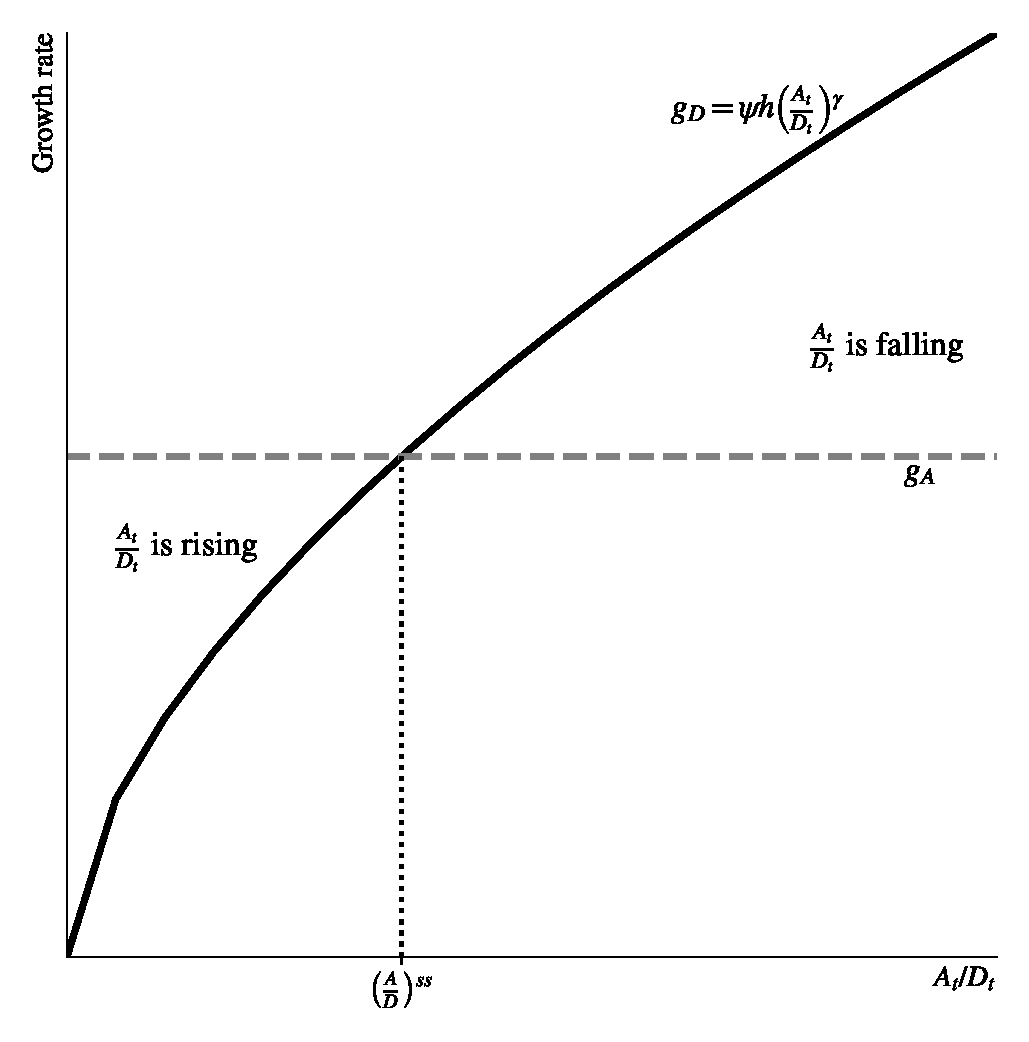
\includegraphics[height=3in]{../Figures/fig-ch7-fig2.eps}
\end{center}
\end{frame}

\begin{frame}{Steady state}
Given any initial ratio $A/D$
\begin{itemize}
	\item The growth rate $g_D = g_A$
	\item Followers can only grow as fast as the leaders
	\item As they catch up they slow down
	\item The level of $D$ determines how close to the frontier a country is
\end{itemize}
\end{frame}

\begin{frame}{Steady state}
What's the steady state $A/D$ ratio?
\begin{equation}
	\left(\frac{A}{D}\right)^{ss} = \left(\frac{g_A}{\psi h}\right)^{1/\gamma}. \label{EQ_DAss}
\end{equation}
This ratio is \textit{smaller} and the follower is \textit{closer} when
\begin{itemize}
	\item $h$ is high. More HC means easier to adopt new technologies
	\item $g_A$ is low. If the leader grows slowly, it's easier to keep up
\end{itemize}
\end{frame}

\begin{frame}{BGP}
At any given point in time the level of $D_t$ is
\begin{equation}
	D_t = \left(\frac{\psi h}{g_A}\right)^{1/\gamma} A_t, 
\end{equation}
which means the BGP for GDP per capita in the follower is
\begin{equation}
	y_t^{BGP} = \left(\frac{s_I}{g_A + g_L + \delta} \right)^{\frac{\alpha}{1-\alpha}} h \left(\frac{\psi h}{g_A}\right)^{1/\gamma} A_t. 
\end{equation}
and the follower runs ``parallel'' to the BGP of the leader.
\end{frame}

\begin{frame}{Human Capital}
Note that with this BGP
\begin{equation}
	y_t^{BGP} = \left(\frac{s_I}{g_A + g_L + \delta} \right)^{\frac{\alpha}{1-\alpha}} h \left(\frac{\psi h}{g_A}\right)^{1/\gamma} A_t. \label{EQ_dev_yBGP}
\end{equation}
\begin{itemize}
	\item Human capital is more important than just via skills ($h$)
	\item The $h^{1/\gamma}$ term influences diffusion
	\item Development accounting may understate importance of human capital
\end{itemize}
\end{frame}

\section{Trade and globalization}
\begin{frame}{Importing ideas}
Think of international trade as a way of importing ideas via varieties. 
\begin{equation}
	Y_t = (h_t L_t)^{1-\alpha} \int_0^{D_t+M_t} x_{jt} dj \label{EQ_final_trade}.
\end{equation}
where $D_t$ are the domestic varieties and $M_t$ are imported varieties. Trade can raise GDP by adding new types of goods. 
\end{frame}

\begin{frame}{Domestic production}
On the domestic side, 
\begin{equation}
	D_tz_t = K_t. \nonumber
\end{equation}
The country uses $K_t$ in capital to produce $z_t$ units of the $D_t$ varieties they can make. 
\begin{equation}
	K_t - D_tx_t = D_t (z_t - x_t)  = M_tx_t. \label{EQ_Kdxmx}
\end{equation}
But the country only \textit{uses} $x_t$ units of those varieties, leaving $D_t(z_t-x_t)$ for export, which are traded for $M_t x_t$ units of foreign varieties. 
\end{frame}

\begin{frame}{Trade balance}
Interpreting the trade:
\begin{itemize}
	\item You can think of $D_t (z_t - x_t)$ as a literal amount of goods shipped to foreign countries.
	\item You can think of $M_t x_t$ as the amount of goods imported from those countries
	\item OR you can think of $D_t (z_t - x_t)$ as capital that is owned by the domestic country in a foreign country (outward FDI)
	\item and then $M_tx_t$ is amount of capital owned by a foreign country in the domestic country (inward FDI) 
\end{itemize}
This assumes balanced trade at all times. Adding deficits or surpluses involves additional work on consumption side. 
\end{frame}

\begin{frame}{Trade and GDP}
Whatever the interpretations we have
\begin{equation}
	K_t = x_t(D_t + M_t), \nonumber
\end{equation}
which allows us to write GDP as
\begin{equation}
	Y_t = K_t^{\alpha}(D_th_tL_t)^{1-\alpha}\left(1+\frac{M_t}{D_t}\right)^{1-\alpha}. \nonumber
\end{equation}
Domestic varieties act like a productivity term. But we also have this $M_t/D_t$ ratio which can boost productivity. Note that
\begin{equation}
	\frac{\text{Imports}}{\text{GDP}} = \frac{M_tx_t}{Y_t} = \frac{M_t}{D_t+M_t}\frac{K_t}{Y_t}
\end{equation}
so if imports/GDP go up, GDP should be higher. Trade is unequivocally good for GDP in this setup due to varieties.
\end{frame}

\begin{frame}{Trade and GDP}
\begin{center}
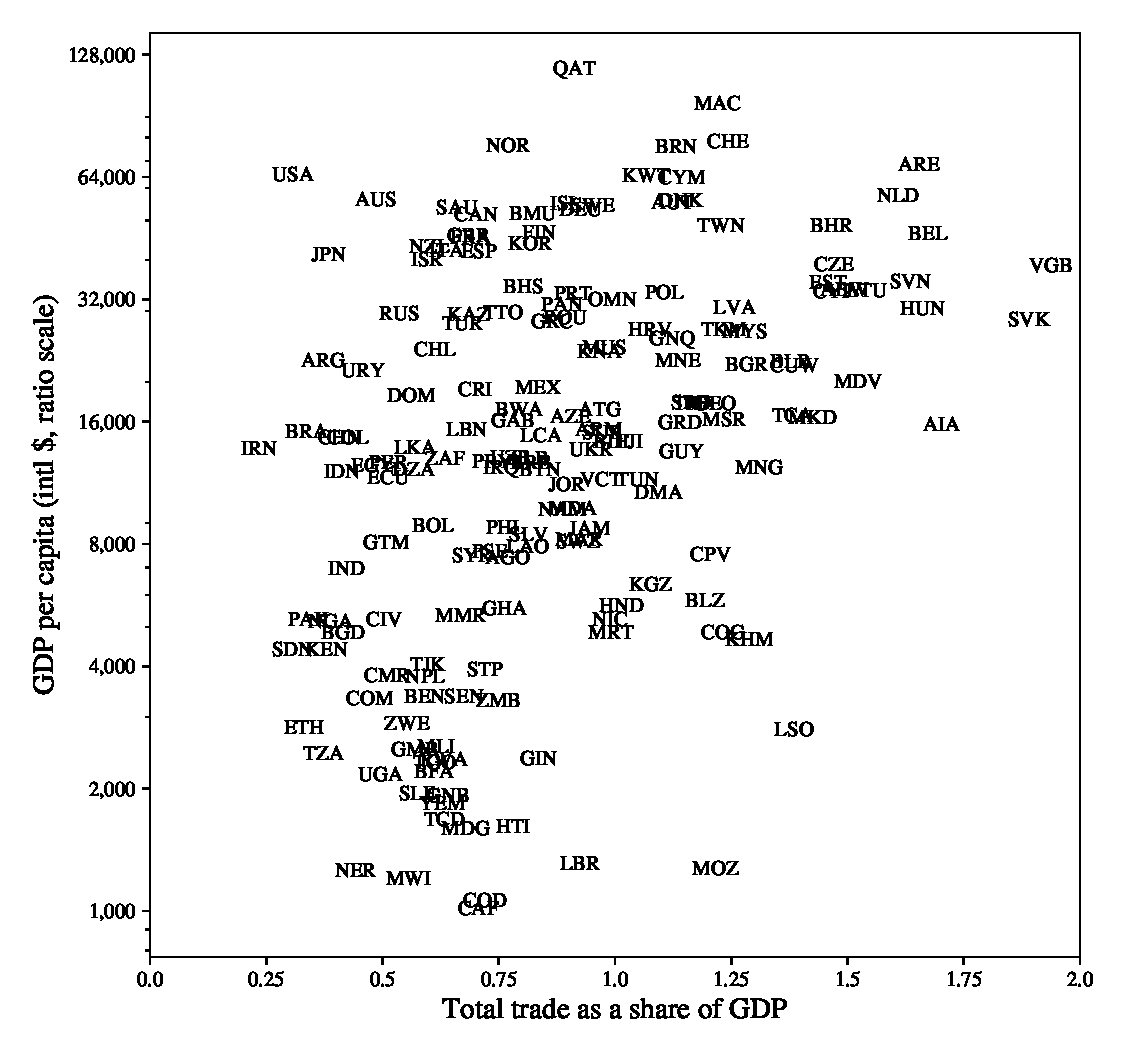
\includegraphics[height=3in]{../Figures/fig-ch7-fig3.eps}
\end{center}
\end{frame}


\section{Misallocation}
\begin{frame}{Factor use}
Alternative way to think about productivity differences is via allocations.
\begin{itemize}
	\item In Romer model, we assumed each variety was ``equal'' in terms of allocation
	\item Each used $K/A$ of the capital stock, because each was equally productive, $x_i = K_i$
	\item But what if some firms/varieties get more capital and some less? 
	\item Lower overall GDP because the marginal product of the varieties would differ
	\item This would show up in measurement as lower aggregate $A$ given the factors used
\end{itemize}
\end{frame}

\begin{frame}{Marginal product}
Let production look like this
\begin{equation}
	Y = L^{1-\alpha} \int_{0}^{D} x_{j}^{\alpha} dj. \label{EQ_final_dev}
\end{equation}
where $D$ are the number of varieties, as usual. What's the marginal product of any given variety?
\begin{equation}
	MP_j = L^{1-\alpha} \alpha x_j^{\alpha-1}
\end{equation}
and as each variety uses capital, $x_j = K_j$, the marginal product is
\begin{equation}
	MP_j = L^{1-\alpha} \alpha K_j^{\alpha-1} = \left(\frac{L}{K_j}\right)^{1-\alpha}
\end{equation}
\end{frame}

\begin{frame}{Compare marginal products}
Take two varieties, $i$ and $j$. If $K_i > K_j$ then 
\begin{itemize}
	\item $MP_i < MP_j$ because MP declines with capital used
	\item Move one unit of capital from $i$ to $j$. You lose $MP_i$, you gain $MP_j$. Net increase in GDP.
	\item If we can raise GDP just be re-allocating capital (not accumulating it) then there is a mis-allocation
	\item Mis-allocations - different MPs - make GDP lower for a given set of $K$, $L$
	\item Therefore mis-allocations must show up as lower measured $A$
\end{itemize}
\end{frame}

\begin{frame}{Why mis-allocations?}
If there are mis-allocations and $MP_i \neq MP_j$, why? 
\begin{itemize}
	\item Capital isn't substitutable. We're wrong that $K_i$ could be used as $K_j$ (office building versus a drill press)
	\item Policies (taxes, subsidies) favor one variety over the other. State-owned enterprises may get cheaper capital, for example.
	\item Transport and relocation costs. It's not possible move an entire factory from Ohio to Alabama.
	\item Differences in market power. $i$ faces competitors, $j$ is a monopolist?
\end{itemize}

\end{frame}

\end{document}